\chapter{Hydras and hydra games}

\label{sec:orgheadline91}
\label{chapter:hydras}




This chapter is dedicated to the representation of hydras and rules of the hydra game in \coq's specification language:~\gallina. 


Technically, a \emph{hydra} is just a finite ordered tree, each node of which 
has any number of sons. Contrary to the computer science tradition, we display the hydras 
with the heads up and the foot (i.e., the root of the tree) down.
Fig.~\ref{fig:Hy} represents such  a hydra, which will be referred to as \texttt{Hy} in our examples (please look at the 
module~\href{../theories/html/hydras.Hydra.Hydra_Examples.html}{Hydra.Hydra\_Examples}). 
\emph{For a less formal description of hydras, please see 
\url{https://www.smbc-comics.com/comic/hydra}.}

\begin{figure}[h]
\centering
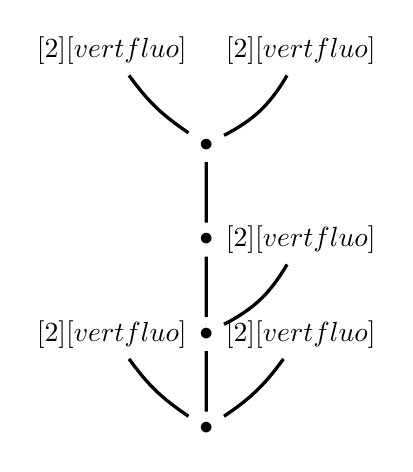
\begin{tikzpicture}[very thick, scale=0.6]

\node (foot) at (2,0) {$\bullet$};
\node (N1) at (2,2) {$\bullet$};
\node (N2) at (2,4) {$\bullet$};
\node (N3) at (2,6) {$\bullet$};
\node (H0) at (0,2) {$\Smiley[2][vertfluo]$};
\node (H1) at (0,8) {$\Smiley[2][vertfluo]$};
\node (H2) at (4,8) {$\Smiley[2][vertfluo]$};
\node (H4) at (4,2) {$\Smiley[2][vertfluo]$};
\node (H5) at (4,4) {$\Smiley[2][vertfluo]$};
\draw (foot) -- (N1)[very thick] ;
\draw (N1) -- (N2);
\draw (N2) -- (N3);
\draw (N3) to [bend left= 10]  (H1) ;
\draw (N3) to [bend right= 16] (H2);
\draw (foot) to [bend left= 10]  (H0) ;
\draw (foot) to [bend right = 10] (H4) ;
\draw (N1) to [bend right= 16] (H5);
\end{tikzpicture}
\caption{The hydra \texttt{Hy} \label{fig:Hy}}
\end{figure}



We use a specific vocabulary for talking about hydras. Table~\ref{tab:hyd2tree} shows the correspondence between our terminology and the usual vocabulary for trees in computer science.


\begin{figure}[h]
  \centering
  \begin{tabular}{ll}
Hydras & Finite rooted trees\\
\hline
foot & root\\
head & leaf\\
node & node\\
segment  & (directed) edge \\
sub-hydra & subtree\\
daughter & immediate subtree\\
\end{tabular}
  \caption{Translation from hydras to trees}
  \label{tab:hyd2tree}
\end{figure}


The hydra \texttt{Hy} has a \emph{foot} (below), five \emph{heads}, and eight \emph{segments}. 
We leave it to the reader to define various parameters such as the height, the size, the highest arity (number of sons of a node) of a hydra. In our example, these parameters have the respective values $4$, $9$ and $3$.




\subsection{The rules of the game}

\label{sec:orgheadline44}
\label{sect:replication-def}

A \emph{hydra battle} is a fight between Hercules and the Hydra. 
More formally, a  battle is a sequence of \emph{rounds}.
At each round:
\begin{itemize}
\item If the hydra is composed of just one head, the battle is finished
and  Hercules is the winner.
\item Otherwise, Hercules chops off \emph{one} head of the hydra,

\begin{itemize}
\item If the head is at distance 1 from the foot, the head is just lost by the hydra, with no more reaction.
\item Otherwise, let us denote by \(r\) the node that was at distance \(2\) from 
the removed head in the direction of the foot,  and consider the  sub-hydra \(h'\) of \(h\), whose  root is \(r\) \footnote{$h'$ will be called ``the wounded part of the hydra'' in the subsequent text. In Figures~\vref{fig:Hy2} and ~\vref{fig:Hy4}, this sub-hydra  is displayed in red.}. Let $n$ be some natural number.
Then $h'$ is replaced by  $n+1$ of copies of \(h'\) which share the same root $r$.
 The \emph{replication factor} $n$ may be different (and generally is)   at each round of the fight.
It may be chosen by the hydra, according to its strategy, or imposed by some 
particular rule. In many presentations of hydra battles, this number is increased by $1$ at each round. In the following presentation, we will also consider battles where the hydra is free to choose its ~replication factor at each round of the battle\footnote{Let us recall that, if the chopped-off head was at distance 1 from the foot, the replication factor is meaningless.}.
\end{itemize}
\end{itemize}



Note that the description given in~\cite{KP82} of the replication process in hydra battles is also  semi-formal. 

\label{original-rules}

\begin{quote}
  ``From the node that used to be attached to the head which was just chopped off, traverse one 
segment towards the root until the next node is reached. From this node sprout $n$ replicas of 
that part of the hydra (after decapitation) which is ``above'' the segment just traversed, i.e., those 
nodes and segments from which, in order to reach the root, this segment would have to be 
traversed. If the head just chopped off had the root of its nodes, no new head is grown. ''
\end{quote}

Moreover, we note that this description is in \emph{imperative} terms. In order to formally study the properties of hydra battles, we prefer to use a mathematical vocabulary, i.e., graphs, relations, functions, etc.
Thus, the replication process will be represented as a binary relation on a data type \texttt{Hydra},
linking the state of the hydra \emph{before} and \emph{after} the transformation.
A battle will thus be represented as a sequence of terms of type \texttt{Hydra}, respecting the rules of the game.





\subsection{Example}
Let us start a battle between Hercules and the hydra \texttt{Hy} of Fig.~\ref{fig:Hy}.

At the first round, Hercules chooses to chop off the rightmost head of \texttt{Hy}.
Since this head is near the floor, the hydra simply loses this head. Let us call 
 \texttt{Hy'} the resulting state of the hydra, represented in Fig.~\vref{fig:Hy-prime}.

Next, assume Hercules chooses to chop off one of the two highest heads of \texttt{Hy'}, for instance the rightmost one. Fig.~\vref{fig:Hy2} represents the broken segment in dashed lines, and the part that will be replicated in red. Assume also that the hydra decides to add 4 copies of the red part\footnote{In other words, the replication factor at this round is equal to $4$.}. We obtain a new state \texttt{Hy''} depicted in Fig.~\ref{fig:Hy3}.



\begin{figure}[h]
\centering
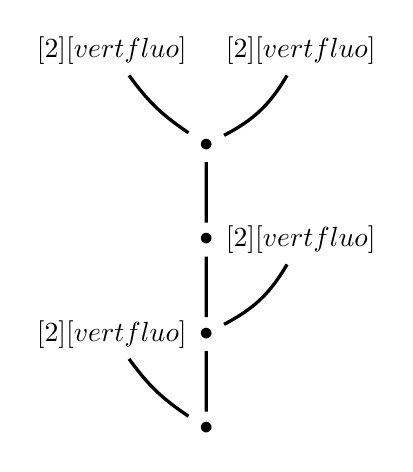
\begin{tikzpicture}[very thick, scale=0.6]

\node (foot) at (2,0) {$\bullet$};
\node (N1) at (2,2) {$\bullet$};
\node (N2) at (2,4) {$\bullet$};
\node (N3) at (2,6) {$\bullet$};
\node (H0) at (0,2) {$\Smiley[2][vertfluo]$};
\node (H1) at (0,8) {$\Smiley[2][vertfluo]$};
\node (H2) at (4,8) {$\Smiley[2][vertfluo]$};
\node (H5) at (4,4) {$\Smiley[2][vertfluo]$};
%\node (H4) at (6,0) {$\Xey[2][lightgray]$};
\draw (foot) -- (N1)[very thick] ;
\draw (N1) -- (N2);
\draw (N2) -- (N3) ;
\draw (N3) to [bend left= 10]  (H1) ;
\draw (N3) to [bend right= 16] (H2);
\draw (foot) to [bend left= 10]  (H0) ;
\draw (N1) to [bend right= 16] (H5);
\end{tikzpicture}

\caption{\texttt{Hy'}: the state  of \texttt{Hy} after one round \label{fig:Hy-prime}}
\end{figure}


\begin{figure}[hp]
\centering
\begin{tikzpicture}[very thick, scale=0.5]

\node (foot) at (2,0) {$\bullet$};
\node (N1) at (2,2) {$\bullet$};
\node (N2) at (2,4)  {{\color{lightred}$\bullet$}};
\node (N3) at (2,6) {{\color{lightred}$\bullet$}};
\node (H0) at (0,2) {$\Smiley[2][vertfluo]$};
\node (H1) at (0,8) {$\Sey[2][lightred]$};
%\node (H2) at (5,0) {$\Xey[2][lightgray]$};
\node (H5) at (4,4) {$\Smiley[2][vertfluo]$};
\node (ex) at (5,8) {};
\draw (foot) -- (N1)[very thick] ;
\draw (N1) -- (N2);
\draw  (N2) -- (N3)[draw=lightred];
\draw (N3) to   [bend left= 10](H1) [draw=lightred];
\draw [dashed] (N3) to [bend left= 10](ex);
\draw (foot) to [bend left= 10]  (H0) ;
\draw (N1) to [bend right= 16] (H5);
\end{tikzpicture}
\caption{A second beheading}
\label{fig:Hy2}
\end{figure}

\begin{figure}[hp]
\centering
\begin{tikzpicture}[very thick, scale=0.6]

\node (foot) at (2,0) {$\bullet$};
\node (N1) at (2,2) {$\bullet$};
\node (N2) at (2,4) {$\bullet$};
\node (N3) at (2,6) {{\color{lightred}$\bullet$}};
\node (H1) at (0,8) {$\Smiley[2][vertfluo]$};
\node (H11) at (2,8) {$\Smiley[2][vertfluo]$};
\node (H12) at (4,8) {$\Smiley[2][vertfluo]$};
\node (H13) at (6,8) {$\Smiley[2][vertfluo]$};
\node (H14) at (8,8) {$\Smiley[2][vertfluo]$};

\node (N3) at (1,6) {$\bullet$};
\node (N31) at (2,6) {$\bullet$};
\node (N32) at (3,6) {$\bullet$};
\node (N33) at (4,6) {$\bullet$};
\node (N34) at (5,6) {$\bullet$};

\node (H0) at (0,2) {$\Smiley[2][vertfluo]$};
\node (H5) at (4,4) {$\Smiley[2][vertfluo]$};
\draw (foot) -- (N1)[very thick] ;
\draw (N1) -- (N2);
\draw (N2) -- (N3);
\draw (N2) -- (N31);
\draw (N2) -- (N32);
\draw (N2) -- (N33);
\draw (N2) -- (N34);
\draw (N3) to   [bend left= 10](H1) ;
\draw (N31) to   [bend left= 10](H11) ;
\draw (N32) to   [bend left= 10](H12) ;
\draw (N33) to   [bend left= 10](H13) ;
\draw (N34) to   [bend left= 10](H14) ;
\draw (foot) to [bend left= 10]  (H0) ;
\draw (N1) to [bend left= 10]  (H5) ;
\end{tikzpicture}
\caption{\texttt{Hy''}: the state of \texttt{Hy} after two rounds \label{fig:Hy3}}
\end{figure}

Figs.~\ref{fig:Hy4} and~\vref{fig:Hy5} represent a possible third round of the battle, with a replication factor equal to $2$. Let us call \texttt{Hy'''} the state of the hydra after that third round.

\begin{figure}[hp]
\centering
\begin{tikzpicture}[very thick, scale=0.6]

\node (foot) at (2,0)  {{\color{lightred}$\bullet$}};
\node (N1) at (2,2) {{\color{lightred}$\bullet$}};
\node (N2) at (2,4) {{\color{lightred}$\bullet$}};
\node (N3) at (2,6) {{\color{lightred}$\bullet$}};
\node (exN4) at (4,4) {};
\node (H1) at (0,8) {$\Sey[2][lightred]$};
\node (H11) at (2,8) {$\Sey[2][lightred]$};
\node (H12) at (4,8) {$\Sey[2][lightred]$};
\node (H13) at (6,8) {$\Sey[2][lightred]$};
\node (H14) at (8,8) {$\Sey[2][lightred]$};

\node (N3) at (1,6) {{\color{lightred}$\bullet$}};
\node (N31) at (2,6) {{\color{lightred}$\bullet$}};
\node (N32) at (3,6) {{\color{lightred}$\bullet$}};
\node (N33) at (4,6) {{\color{lightred}$\bullet$}};
\node (N34) at (5,6) {{\color{lightred}$\bullet$}};

\node (H0) at (0,2) {$\Smiley[2][vertfluo]$};
%\node (H5) at (4,0) {$\Xey[2][lightgray]$};
\draw (foot) -- (N1)[very thick,draw=lightred] ;
\draw (N1) -- (N2)[draw=lightred];
\draw (N2) -- (N3)[draw=lightred];
\draw (N2) -- (N31)[draw=lightred];
\draw (N2) -- (N32)[draw=lightred];
\draw (N2) -- (N33)[draw=lightred];
\draw (N2) -- (N34)[draw=lightred];
\draw (N3) to   [bend left= 10](H1) [draw=lightred];
\draw (N31) to   [bend left= 10](H11) [draw=lightred];
\draw (N32) to   [bend left= 10](H12) [draw=lightred];
\draw (N33) to   [bend left= 10](H13) [draw=lightred];
\draw (N34) to   [bend left= 10](H14) [draw=lightred];
\draw (foot) to [bend left= 10]  (H0) ;
\draw [dashed] (N1) to  [bend left= 10](exN4);
\end{tikzpicture}
\caption{A third beheading (wounded part in red) \label{fig:Hy4}}
\end{figure}

\begin{figure}[hp]
\centering
\begin{tikzpicture}[very thick, scale=0.4]

\node (foot) at (10,0) {$\bullet$};


\node (N1) at (2,2) {$\bullet$};
\node (N2) at (2,4) {$\bullet$};
\node (N3) at (2,6) {{\color{lightred}$\bullet$}};
\node (H1) at (0,8) {$\Smiley[1][vertfluo]$};
\node (H11) at (2,8) {$\Smiley[1][vertfluo]$};
\node (H12) at (4,8) {$\Smiley[1][vertfluo]$};
\node (H13) at (6,8) {$\Smiley[1][vertfluo]$};
\node (H14) at (8,8) {$\Smiley[1][vertfluo]$};

\node (N3) at (1,6) {$\bullet$};
\node (N31) at (2,6) {$\bullet$};
\node (N32) at (3,6) {$\bullet$};
\node (N33) at (4,6) {$\bullet$};
\node (N34) at (5,6) {$\bullet$};

\node (H0) at (-3,3) {$\Smiley[1][vertfluo]$};

\draw (foot) to [bend left=10] (N1)[very thick] ;
\draw (N1) -- (N2);
\draw (N2) -- (N3);
\draw (N2) -- (N31);
\draw (N2) -- (N32);
\draw (N2) -- (N33);
\draw (N2) -- (N34);
\draw (N3) to   [bend left= 10](H1) ;
\draw (N31) to   [bend left= 10](H11) ;
\draw (N32) to   [bend left= 10](H12) ;
\draw (N33) to   [bend left= 10](H13) ;
\draw (N34) to   [bend left= 10](H14) ;
\draw (foot) to [bend left = 15]  (H0) ;


% second copy 
\node (N01) at (12,2) {$\bullet$};
\node (N02) at (12,4) {$\bullet$};
\node (N03) at (12,6) {{\color{lightred}$\bullet$}};
\node (H001) at (10,8) {$\Smiley[1][vertfluo]$};
\node (H0011) at (12,8) {$\Smiley[1][vertfluo]$};
\node (H0012) at (14,8) {$\Smiley[1][vertfluo]$};
\node (H0013) at (16,8) {$\Smiley[1][vertfluo]$};
\node (H0014) at (18,8) {$\Smiley[1][vertfluo]$};

\node (N03) at (11,6) {$\bullet$};
\node (N031) at (12,6) {$\bullet$};
\node (N032) at (13,6) {$\bullet$};
\node (N033) at (14,6) {$\bullet$};
\node (N034) at (15,6) {$\bullet$};

\draw (foot) -- (N01)[very thick] ;
\draw (N01) -- (N02);
\draw (N02) -- (N03);
\draw (N02) -- (N031);
\draw (N02) -- (N032);
\draw (N02) -- (N033);
\draw (N02) -- (N034);
\draw (N03) to   [bend left= 10](H001) ;
\draw (N031) to   [bend left= 10](H0011) ;
\draw (N032) to   [bend left= 10](H0012) ;
\draw (N033) to   [bend left= 10](H0013) ;
\draw (N034) to   [bend left= 10](H0014) ;

% third copy 
\node (N001) at (22,2) {$\bullet$};
\node (N002) at (22,4) {$\bullet$};
\node (N003) at (22,6) {{\color{lightred}$\bullet$}};
\node (H001) at (20,8) {$\Smiley[1][vertfluo]$};
\node (H0011) at (22,8) {$\Smiley[1][vertfluo]$};
\node (H0012) at (24,8) {$\Smiley[1][vertfluo]$};
\node (H0013) at (26,8) {$\Smiley[1][vertfluo]$};
\node (H0014) at (28,8) {$\Smiley[1][vertfluo]$};

\node (N003) at (21,6) {$\bullet$};
\node (N0031) at (22,6) {$\bullet$};
\node (N0032) at (23,6) {$\bullet$};
\node (N0033) at (24,6) {$\bullet$};
\node (N0034) at (25,6) {$\bullet$};

\draw (foot) -- (N001)[very thick] ;
\draw (N001) -- (N002);
\draw (N002) -- (N003);
\draw (N002) -- (N0031);
\draw (N002) -- (N0032);
\draw (N002) -- (N0033);
\draw (N002) -- (N0034);
\draw (N003) to   [bend left= 10](H001) ;
\draw (N0031) to   [bend left= 10](H0011) ;
\draw (N0032) to   [bend left= 10](H0012) ;
\draw (N0033) to   [bend left= 10](H0013) ;
\draw (N0034) to   [bend left= 10](H0014) ;
\end{tikzpicture}
\caption{The configuration \texttt{Hy'''} of \texttt{Hy} \label{fig:Hy5}}
\end{figure}
\FloatBarrier

We leave it to the reader  to guess the following  rounds of the battle \dots
 % Please keep in mind that, in this 
% the hydra is free to chose any number of replications at each time, whereas
% Hercules chops only one head per round.

% Let us precise that, in this game, Hercules wins if the hydra is eventually reduced 
% to a single head. 
% We know from~\cite{KP82} that, whichever the initial configuration of the
% hydra, and the strategies of both players, Hercules eventually wins. The 
% aforementionned paper shows also that there do not exist any \emph{simple} proof of this result.


\section{Hydras and their representation in \emph{Coq}}
\label{sec:orgheadline48}

\index{hydras}{Library Hydra!Types!Hydra}
\index{hydras}{Library Hydra!Types!Hydrae}


In order to describe trees where each node can have an arbitrary (but finite) number of sons, it is usual to define a type where each node carries a \emph{forest}, \emph{i.e} a list of trees
(see for instance Chapter 14, pages 400-406 of \cite{BC04}, also available as~\cite{BC04ch14}).

For this purpose, we define two mutual \emph{ad-hoc}  inductive types, where \texttt{Hydra} is the main type, and \texttt{Hydrae} is a helper for describing finite sequences of hydras.
\label{types:Hydra}
\label{types:Hydrae}

\vspace{4pt}
\noindent
\emph{From Module~\href{../theories/html/hydras.Hydra.Hydra_Definitions.html\#Hydra}{Hydra.Hydra\_Definitions}}

\input{movies/snippets/Hydra_Definitions/HydraDef}


%\index{To do}
\index{hydras}{Projects}

\begin{project}
Look for an existing library on trees with nodes of arbitrary arity, in order to replace  this ad-hoc type with something more generic.
\end{project}


%\index{hydras}{Projects}

\begin{remark}[Mutually inductive types vs lists of hydras]
\label{hydra:mutually-inductive-vs-lists}
 Another very similar representation could use the \texttt{list} type family instead of the specific 
type \texttt{Hydrae}:


\input{movies/snippets/Hydra_Definitions/HydraAlt}

Using this representation, one can re-define all the constructions of this chapter, which is left as an exercise.
You will probably have to use patterns described for instance in~\cite{BC04} or the archives of the \coq communication channels (please consult~\url{https://coq.inria.fr/community.html}).

  
\end{remark}


\index{hydras}{Projects}

\begin{project}
  Our type \texttt{Hydra} describes hydras as
  \emph{plane oriented trees}, i.e., as drawn on a sheet of paper or computer screen. Thus, it is appropriate to consider a \emph{leftmost} or \emph{rightmost} head of
the beast. It could be interesting to consider another representation, in which
every non-leaf node has a \emph{multi-set} -- not an ordered list -- of daughters.
\end{project}

\subsubsection{Abbreviations}

We provide several notations for hydra patterns  which occur often in our developments. 

\vspace{4pt}
\noindent
\emph{From Module~\href{../theories/html/hydras.Hydra.Hydra_Definitions.html\#head}{Hydra.Hydra\_Definitions}}


\input{movies/snippets/Hydra_Definitions/headsEtc}

For instance, the hydra \texttt{Hy}  of Figure~\vref{fig:Hy} is defined as follows:

\vspace{4mm}
\noindent
\emph{From Module~\href{../theories/html/hydras.Hydra.Hydra_Examples.html\#Hy}{Hydra.Hydra\_Examples}}

\input{movies/snippets/Hydra_Examples/Hy}



Hydras quite frequently contain  multiple adjacent  copies of the same subtree. The following functions
will help us to describe and reason about replications in hydra battles.

\vspace{4pt}
\noindent
\emph{From Module~\href{../theories/html/hydras.Hydra.Hydra_Definitions.html\#hcons_mult}{Hydra.Hydra\_Definitions}}

\input{movies/snippets/Hydra_Definitions/hconsMult}



\vspace{4mm}

Let us consider for instance the hydra \texttt{Hy''} of Fig~\vref{fig:Hy3}.

\vspace{4pt}
\noindent
\emph{From Module~\href{../theories/html/hydras.Hydra.Hydra_Examples.html}{Hydra.Hydra\_Examples}}

\input{movies/snippets/Hydra_Examples/HySecond}






\subsubsection{Recursive functions on type \texttt{Hydra}}
\label{sec:orgheadline41}
\label{sec:hsize-def}




In order to  define a recursive function over the type \texttt{Hydra}, one has to consider the three constructors 
\texttt{node}, \texttt{hnil} and \texttt{hcons} of the mutually inductive types \texttt{Hydra} and \texttt{Hydrae}. 
Let us define for instance the function which  computes the number of nodes of any hydra:

\vspace{4pt}
\noindent
\emph{From Module~\href{../theories/html/hydras.Hydra.Hydra_Definitions.html}{Hydra.Hydra\_Definitions}}

\input{movies/snippets/Hydra_Definitions/hsize}

\input{movies/snippets/Hydra_Examples/HySize}


Likewise, the \emph{height} (maximum distance between the foot and a head) 
is defined by mutual recursion:

\input{movies/snippets/Hydra_Definitions/height}

\input{movies/snippets/Hydra_Examples/HyHeight}



\index{hydras}{Exercises}

\begin{exercise}
Define a function \texttt{max\_degree: Hydra $\arrow$ nat} which  returns the highest degree of a node in any hydra. For instance, the evaluation of the term \texttt{(max\_degree Hy)} should return $3$.
\end{exercise}

\subsection{Induction principles for hydras}
\label{sec:orgheadline42}


In this section, we show how induction principles are used to prove properties on the type 
\texttt{Hydra}. Let us consider for instance the following statement:
\begin{quote}
  `` The height of any hydra is strictly less than its size. ''
\end{quote}



\subsubsection{A failed attempt}

One may try to use the default tactic of proof by induction, which corresponds to an application of the automatically  generated  induction principle for  type \texttt{Hydra}:

\input{movies/snippets/Hydra_Examples/HydraInd}

Let us start a simple proof by induction.

\vspace{4pt}
\noindent
\emph{From Module~\href{../theories/html/hydras.Hydra.Hydra_Examples.html}{Hydra.Hydra\_Examples}}

\input{movies/snippets/Hydra_Examples/BadInductiona}



We might be tempted to do an induction on the sequence \texttt{s}:

\input{movies/snippets/Hydra_Examples/BadInductionb}

The first subgoal is trivial.

\input{movies/snippets/Hydra_Examples/BadInductionc}

Let us look now at the second subgoal of the induction.

\input{movies/snippets/Hydra_Examples/BadInductiond}

We notice that this sub-goal does not contain any hypothesis
on the height and size of the hydra \texttt{h}. So, it looks hard to prove the conclusion. Let's stop.

\input{movies/snippets/Hydra_Examples/BadInductione}

\subsubsection{A Principle of mutual induction}
In order to get an appropriate induction scheme for the types 
\texttt{Hydra} and \texttt{Hydrae}, we can use  \coq{}'s  command \texttt{Scheme}.


\index{coq}{Mutually inductive types}
%\index{coq}{Commands!Scheme}

\input{movies/snippets/Hydra_Definitions/HydraRect2}

\input{movies/snippets/Hydra_Examples/HydraRect2Check}





\subsubsection{A Correct proof}

Let us now use \texttt{Hydra\_rect2} for proving that the height of any hydra is strictly less than its size.
Using this scheme requires an auxiliary predicate, called \texttt{P0} in \texttt{Hydra\_rect2}'s statement. 

\vspace{4pt}
\noindent
\emph{From Module~\href{../theories/html/hydras.Hydra.Hydra_Definitions.html}{Hydra.Hydra\_Definitions}}

\input{movies/snippets/Hydra_Definitions/hForall}

\emph{From Module~\href{../theories/html/hydras.Hydra.Hydra_Examples.html}{Hydra.Hydra\_Examples}}
\input{movies/snippets/Hydra_Examples/heightLtSizea}




The first subgoal is easily solvable, using some arithmetic.
The second and third ones are
almost trivial. We let the reader look at the source. 
\input{movies/snippets/Hydra_Examples/heightLtSizez}



\index{hydras}{Exercises}

\begin{exercise}
It happens very often that, in the proof of  a proposition of the form 
(\texttt{$\forall\,$ h:Hydra, $P$ h}), the predicate \texttt{P0}
is  (\texttt{h\_forall $P$}).  Design a tactic for induction on hydras that frees the user from binding explicitly \texttt{P0},  and solves trivial subgoals. Apply it for writing  a shorter proof script of \texttt{height\_lt\_size}.
\end{exercise}
 


\section{Relational description of hydra battles}


In this section, we represent the rules of hydra battles as a binary relation associated with
a \emph{round}, i.e., an interaction composed of the two following actions:
\begin{enumerate}
\item Hercules chops off one head of the hydra.
\item Then, the  hydra replicates the wounded part (if the head is at distance $\geq 2$ from the foot).
\end{enumerate}
The relation associated with each round of the battle is parameterized  by the \emph{expected} replication  factor (irrelevant if the chopped head is at distance 1 from the foot,
but present for consistency's sake).

In our description,  we will apply the following naming convention: if $h$ represents the configuration of the hydra before a round, then the configuration of $h$ after this round will be called $h'$.
 Thus, we are going to define a proposition  (\texttt{round\_n $n\;h\;h'$})  whose intended meaning will be `` the hydra $h$  is transformed into $h'$  in a single round of a battle, with the expected replication factor $n$ ''.


Since the replication of parts of the hydra depends on the distance of the chopped head from  the foot, we  decompose our description into two main  cases, under the form of a bunch of [mutually] inductive predicates over the types \texttt{Hydra} and \texttt{Hydrae}.

The mutually exclusive cases we consider are the following:
\begin{itemize}
\item \textbf{R1}: The chopped off head was at distance 1 from the foot.
\item \textbf{R2}: The chopped off head was at a distance greater than or equal to  $2$ from the foot.
\end{itemize}



\subsection{Chopping off a head at distance 1 from the foot (relation  R1)}

If Hercules chops off a head close to the root, there is no replication at all. We use an auxiliary 
predicate \texttt{S0}, associated with the removing of one head from a sequence of hydras.


\vspace{4pt}\emph{From Module\href{../theories/html/hydras.Hydra.Hydra_Definitions.html}{Hydra.Hydra\_Definitions}}

\input{movies/snippets/Hydra_Definitions/S0Def}
\input{movies/snippets/Hydra_Definitions/R1Def}

\subsubsection{Example}
\label{sec:orgheadline45}

Let us represent in \coq{}   the transformation of the hydra of Fig.~\vref{fig:Hy} into
the configuration represented in Fig.~\ref{fig:Hy-prime}.

\vspace{4pt}
\emph{From Module~\href{../theories/html/hydras.Hydra.Hydra_Examples.html}{Hydra.Hydra\_Examples}}


\input{movies/snippets/Hydra_Examples/Hy1}


\subsection{Chopping off a head at distance \texorpdfstring{$\geq 2$}{>= 2} from the foot (relation R2) }


Let us now consider beheadings  where the chopped-off head is at distance greater than or equal to $2$ from the foot. All the following relations are parameterized by the replication factor  $n$.

 Let $s$ be a sequence of hydras. 
The proposition (\texttt{S1 n s s'}) holds if $s'$ is obtained by replacing some element $h$ of $s$ by 
$n+1$ copies of $h'$, where  the proposition (\texttt{R1 h h'}) holds, in other words, $h'$ is just $h$, without the chopped-off  head. \texttt{S1} is an inductive relation with two constructors that allow us to choose the position in $s'$ of the wounded sub-hydra $h$.

\vspace{4pt}
\noindent
\emph{From Module~\href{../theories/html/hydras.Hydra.Hydra_Definitions.html\#S1}{Hydra.Hydra\_Definitions}}

\input{movies/snippets/Hydra_Definitions/S1Def}


The rest of the definition is composed of two mutually inductive relations on hydras and sequences of hydras. The first constructor of \texttt{R2} describes the case where the chopped head is exactly at height $2$. The others constructors allow us to consider beheadings at height strictly greater than $2$.


\vspace{4pt}
\emph{From Module~\href{../theories/html/hydras.Hydra.Hydra_Definitions.html\#R2}{Hydra.Hydra\_Definitions}}

\input{movies/snippets/Hydra_Definitions/R2Def}

\subsubsection{Example}
Let us prove the transformation of \texttt{Hy'} into \texttt{Hy''} (see Fig.~\vref{fig:Hy3}). We use an experimental set of tactics\footnote{See the \texttt{Ltac} definitions in~\href{../theories/html/hydras.Hydra.Hydra_Definitions.html\#R2}{Hydra.Hydra\_Definitions.}}  for specifying the place where the 
interaction between Hercules and the hydra holds. 


\vspace{4pt}\emph{From Module~\href{../theories/html/hydras.Hydra.Hydra_Examples.html}{Hydra.Hydra\_Examples}}. 

\input{movies/snippets/Hydra_Examples/R2Example}


The reader is encouraged to look at all the successive subgoals of this example.
\emph{Please consider also exercise~\vref{exo:interactive-battle}.}


\subsection{Binary relation associated with a round}

Let us merge \texttt{R1} and \texttt{R1}  into a single relation.
First,  we define the  relation \texttt{(round\_n n h h')} where \texttt{n} is the expected number of  replications (irrelevant in the case of an \texttt{R1}-transformation).
Then, we define a \emph{round} (small step) of a battle
by abstraction over \texttt{n}, 

\vspace{4pt}
\emph{From Module~\href{../theories/html/hydras.Hydra.Hydra_Definitions.html\#round_n}{Hydra.Hydra\_Definitions}}

\index{hydras}{Library Hydra!Predicates!round\_n}
\index{hydras}{Library Hydra!Predicates!round}
\label{sect:infix-round}

\inputsnippets{Hydra_Definitions/roundNDef, Hydra_Definitions/roundDef}





\index{hydras}{Projects}

\begin{project}
Give a direct translation of Kirby and Paris's description of hydra battles (quoted on page~\pageref{original-rules}) and prove that our relational description is consistent with theirs.
\end{project}


\subsection{Rounds and battles}


Using library \href{https://coq.inria.fr/distrib/current/stdlib/Coq.Relations.Relation_Operators.html}{Relations.Relation\_Operators}, we define \texttt{round\_plus},  the transitive closure of \texttt{round}, and \texttt{round\_star},  the reflexive and transitive closure of \texttt{round}.

\label{sect:infix-rounds} 

\input{movies/snippets/Hydra_Definitions/roundPlus}

\index{hydras}{Exercises}

\begin{exercise}
  Prove that if \texttt{$h$ -+-> $h'$}, then
  the height of $h'$ is less or equal than the height of $h$.

\end{exercise}

\begin{remark}
\label{remark:transitive-closure}
\coq's library \href{https://coq.inria.fr/distrib/current/stdlib/Coq.Relations.Relation_Operators.html}{Coq.Relations.Relation\_Operators} 
contains three logically equivalent definitions of the transitive closure of a binary relation. This equivalence is proved in 
\href{https://coq.inria.fr/distrib/current/stdlib/Coq.Relations.Operators_Properties.html}{Coq.Relations.Operators\_Properties} . 

Why three definitions for a single mathematical concept?
Each definition generates an associated induction principle. 
 According to the form of statement one would like to prove, there is a ``best choice'':

\begin{itemize}
\item To prove $\forall y, x\,R^+\,y \;\arrow\; P\,y$, prefer 
\texttt{clos\_trans\_n1}
\item To prove proving $\forall x,\,x\,R^+\,y \;\arrow\; P\,x$, prefer \texttt{clos\_trans\_1n}
\item To prove $\forall x\,y, \,x\,R^+\,y \;\arrow\;P\,x\,y$,  
prefer \texttt{clos\_trans},
\end{itemize}
But there is no ``wrong choice'' at all: the equivalence lemmas in \linebreak 
\href{https://coq.inria.fr/distrib/current/stdlib/Coq.Relations.Operators_Properties.html}{Coq.Relations.Operators\_Properties} 
 allow the user
to convert any one of the three closures into another one before applying the corresponding elimination tactic.
The same remark also holds for reflexive and transitive closures. 
\end{remark}

\index{hydras}{Exercises}

\begin{exercise}
Define a restriction of \coqsimple{round},  where Hercules always chops off
the leftmost among the lowest heads.

Prove that, if $h$ is not a simple head, then there exists a unique $h'$ such that $h$  is transformed into $h'$ in one round, according to this restriction.


\end{exercise}

\index{hydras}{Exercises}

\begin{exercise}[Interactive battles]
\label{exo:interactive-battle}
Given a hydra \texttt{h}, the specification of a hydra battle for \texttt{h} is the type 
\Verb@{h':Hydra | h -*-> h'}@. In order to avoid long sequences of \texttt{split}, \texttt{left}, and 
\texttt{right}, design a set of dedicated tactics for the interactive building of a battle.
Your tactics will have the following functionalities:
\begin{itemize}
\item  Choose to stop a battle, or continue
\item Choose an expected number of replications
\item Navigate in a hydra, looking for a head to chop off.
\end{itemize}

Use your tactics for simulating a small part of a hydra battle, for instance the rounds which lead from
\texttt{Hy} to \texttt{Hy'''}  (Fig.~\vref{fig:Hy5}).

\textbf{Hints:} 
\begin{itemize}

\item Please keep in mind that the last  configuration of your interactively built battle is known only at the end of the battle. Thus, you will have to create and solve subgoals with existential variables. For that purpose, the tactic \texttt{eexists}, applied to the 
goal \Verb@{h':Hydra | h -*-> h'}@ generates the subgoal \Verb|h -*-> ?h'|.
\item You may use Gérard Huet's \emph{zipper} data structure~\cite{zipper} for writing tactics associated with Hercules's  interactive search for a head to chop off.
\end{itemize}






\end{exercise}




\subsection{Classes of battles}
\label{sect:battle-classes}

In some presentations of hydra battles, e.g.~\cite{KP82, bauer2008}, the transformation associated with the $i$-th round may depend on $i$. For instance, in these articles, the replication factor at the $i$-th round is equal to $i$. In other examples, one can allow the hydra to apply any replication factor at any time. In order to be the most general as possible, we define the type of predicates which relate the state of the hydra before and after the $i$-th round of a battle.

\vspace{6pt}
\noindent
\emph{From Module~\href{../theories/html/hydras.Hydra.Hydra_Definitions.html}{Hydra.Hydra\_Definitions}}
\label{types:Battle}
\index{hydras}{Library Hydra!Type classes!Battle}

\input{movies/snippets/Hydra_Definitions/BattleDef}

The most general class of battles is \texttt{free}, which allows the hydra to choose any replication factor at every step:

\vspace{6pt}
\noindent
\emph{From Module~\href{../theories/html/hydras.Hydra.Hydra_Definitions.html\#free}{Hydra.Hydra\_Definitions}}

\input{movies/snippets/Hydra_Definitions/freeDef}

We chose to call \emph{standard}\footnote{This appellation is ours. If there is a better one, we will change it.} the kind of battles which appear  most often in the literature and correspond to an arithmetic progression of the replication factor : $0,1,2,3, \dots$


\vspace{6pt}
\noindent
\emph{From Module~\href{../theories/html/hydras.Hydra.Hydra_Definitions.html\#standard}{Hydra.Hydra\_Definitions}}
\input{movies/snippets/Hydra_Definitions/standardDef}



\subsection{Big steps}

Let $B$ be any instance of class \texttt{Battle}. It is easy to define inductively the relation between the $i$-th and the $j$-th steps of a battle of type $B$. 

\vspace{6pt}
\noindent\emph{From Module~\href{../theories/html/hydras.Hydra.Hydra_Definitions.html\#fight}{Hydra.Hydra\_Definitions}}

\input{movies/snippets/Hydra_Definitions/battleRelDef}

The following property allows us to build battle rounds by composition of smaller ones.

%% TODO display subgoals when fixed

\vspace{6pt}
\noindent\emph{From Module~\href{../theories/html/hydras.Hydra.Hydra_Lemmas.html}{Hydra.Hydra\_Lemmas}}
\noindent
\input{movies/snippets/Hydra_Lemmas/battleTrans}


\section{A long battle}
\label{sect:big-battle}


In this section we consider a simple example of battle, starting with a small hydra,
shown on figure~\vref{fig:hinit}, with a simple strategy for both players:

\begin{itemize}
\item At each round, Hercules chops off the rightmost head of the hydra.
\item The battle is {standard}: at the round number $i$, the expected replication factor is $i$.
\end{itemize}



\begin{figure}[h]
  \centering
  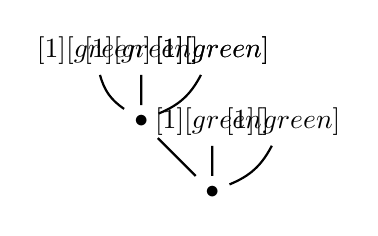
\begin{tikzpicture}[thick, scale=0.30]
 \node (foot) at (6,0) {$\bullet$};
\node (n1) at  (3,3) {$\bullet$};
\node (h1) at  (1,6) {$\Smiley[1][green]$};
\node (h2) at  (3,6) {$\Smiley[1][green]$};
\node (h3) at  (6,6) {$\Smiley[1][green]$};
\node (h4) at  (6,6) {$\Smiley[1][green]$};
\node (h5) at  (6,3) {$\Smiley[1][green]$};
\node (h6) at  (9,3) {$\Smiley[1][green]$};
\draw (foot) -- (n1);
\draw (n1) to   [bend left=20] (h1);
\draw (n1) to   (h2);
\draw (n1) to   [bend right=20] (h3);
\draw (foot) -- (h5);
\draw (foot) to  [bend right=20] (h6);
\end{tikzpicture}

  \caption{The hydra \texttt{hinit}}
  \label{fig:hinit}
\end{figure}

\emph{From Module~\href{../theories/html/hydras.Hydra.BigBattle.html}{Hydra.BigBattle}}

\input{movies/snippets/BigBattle/hinitDef}


The lemma we would like to prove is ``The considered battle lasts exactly $N$ rounds'',
with $N$ being a natural number we have to guess.

But the  battle is so long that no \emph{test} can give us any estimation of its length. Nevertheless, in order to  guess this length, we made some experiments, computing with \gallina{}, \coq{}'s  functional programming language.
Thus, we can consider this development as a collaboration of proof with computation.
In the rest of this section, we show how we found experimentally the value of the number $N$.
The complete proof is in file \url{../theories/html/hydras.Hydra.BigBattle.html}. 

\subsection{First rounds}
During the two first rounds, our hydra loses its two rightmost heads.  Figure~\vref{fig:hinit-plus2} shows the state of the hydra   just before the third round.


\begin{figure}[h]
  \centering
  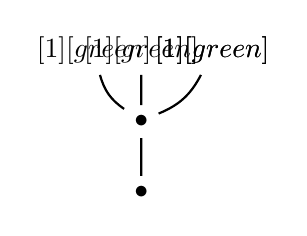
\begin{tikzpicture}[thick, scale=0.30]
 \node (foot) at (3,0) {$\bullet$};
\node (n1) at  (3,3) {$\bullet$};
\node (h1) at  (1,6) {$\Smiley[1][green]$};
\node (h2) at  (3,6) {$\Smiley[1][green]$};
\node (h3) at  (6,6) {$\Smiley[1][green]$};
\node (h4) at  (6,6) {$\Smiley[1][green]$};
\draw (foot) -- (n1);
\draw (n1) to   [bend left=20] (h1);
\draw (n1) to   (h2);
\draw (n1) to   [bend right=20] (h3);
\end{tikzpicture}

  \caption{The hydra (\texttt{hyd1 h3})}
  \label{fig:hinit-plus2}
\end{figure}

The following lemma  is a formal description of these first rounds, in terms of the \texttt{rounds} predicate.


\input{movies/snippets/BigBattle/L02}


\subsection{Looking for regularities}


A first study with pencil and paper suggested us that, after three rounds, the hydra always looks like in figure~\vref{fig:hinit-plusn} (with a variable number of 
subtrees of height 1 or 0).
Thus, we introduce a few handy abbreviations.

\input{movies/snippets/BigBattle/Notations}


For instance, the hydra shown in  Fig~\ref{fig:hinit-plusn} is  (\texttt{hyd 3 4 2}). The hydra (\texttt{hyd 0 0 0})  is the ``final'' hydra of any terminating battle, {i.e.},
a tree whith exactly one node and no edge.

\begin{figure}[h]
  \centering
  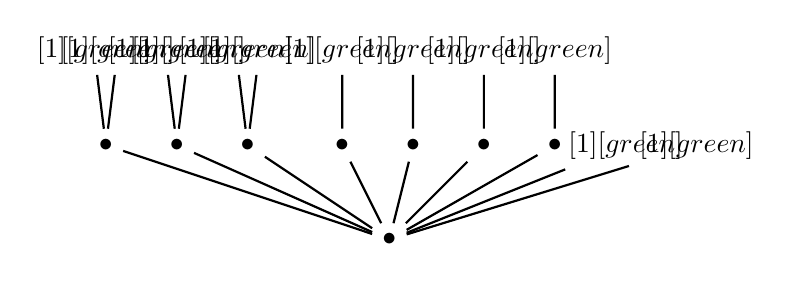
\begin{tikzpicture}[thick, scale=0.30]
 \node (foot) at (15,0) {$\bullet$};
\node (a) at  (3,4) {$\bullet$};
\node (b) at  (6,4) {$\bullet$};
\node (c) at  (9,4) {$\bullet$};
\node (d) at  (13,4) {$\bullet$};
\node (e) at  (16,4) {$\bullet$};
\node (f) at  (19,4) {$\bullet$};
\node (g) at  (22,4) {$\bullet$};
\node (h) at  (25,4) {$\Smiley[1][green]$};
\node (i) at  (28,4) {$\Smiley[1][green]$};
\node (aa) at  (2.5,8) {$\Smiley[1][green]$};
\node (ab) at  (3.5,8) {$\Smiley[1][green]$};
\node (ba) at  (5.5,8) {$\Smiley[1][green]$};
\node (bb) at  (6.5,8) {$\Smiley[1][green]$};
\node (ca) at  (8.5,8) {$\Smiley[1][green]$};
\node (cb) at  (9.5,8) {$\Smiley[1][green]$};
\node (da) at  (13,8) {$\Smiley[1][green]$};
\node (ea) at  (16,8) {$\Smiley[1][green]$};
\node (fa) at  (19,8) {$\Smiley[1][green]$};
\node (ga) at  (22,8) {$\Smiley[1][green]$};
\draw (foot) -- (a);
\draw (foot) -- (b);
\draw (foot) -- (c);
\draw (foot) -- (d);
\draw (foot) -- (e);
\draw (foot) -- (f);
\draw (foot) -- (g);
\draw (foot) -- (h);
\draw (foot) -- (i);
\draw (a) -- (aa);
\draw (a) -- (ab);
\draw (b) -- (ba);
\draw (b) -- (bb);
\draw (c) -- (ca);
\draw (c) -- (cb);
\draw (d) -- (da);
\draw (e) -- (ea);
\draw (f) -- (fa);
\draw (g) -- (ga);
\end{tikzpicture}

  \caption{The hydra (\texttt{hyd 3 4 2})}
  \label{fig:hinit-plusn}
\end{figure}


With these notations, we get a formal description of the first three rounds.

\input{movies/snippets/BigBattle/L23L03}


\subsection{Testing  \dots}
\label{sect:testing}
In order to study \emph{experimentally} the different  configurations of the  battle, we will use a simple data type for representing the states as tuples composed of
the round number, and the respective number of daughters  \texttt{h2}, \texttt{h1}, and heads
of the current hydra.


\input{movies/snippets/BigBattle/stateDef}



The following function returns the next configuration of the game.
Note that this function is defined only for making experiments and is not  ``certified''.  Formal proofs about our battle only start with the lemma
\texttt{step\_rounds}, page~\pageref{lemma:step-battle}.

\input{movies/snippets/BigBattle/nextDef}



We can make bigger steps through iterations of \texttt{next}.
The functional \texttt{iterate}, similar to Standard Library's \texttt{Nat.iter},
is defined and studied in~\href{../theories/html/hydras.Prelude.Iterates.html\#iterate}{Prelude.Iterates}.
\index{hydras}{Library Prelude!iterate}

\label{Functions:iterate}

\input{movies/snippets/Iterates/iterateDef}


The following function computes the state of the battle at the $n$-th round.

\input{movies/snippets/BigBattle/testDefTests}

The battle we are studying looks to be awfully long. Let us concentrate our
tests on some particular events : the states where $\texttt{nh}=0$.
From the value of \texttt{test 5},  it is obvious that at the 10-th round, the counter \texttt{nh} is equal to zero.


\input{movies/snippets/BigBattle/smartTest}

Thus, $(1 + 11)$ rounds later, the \texttt{n1} field is equal to $2$, and 
\texttt{nh}   to $0$. 

\input{movies/snippets/BigBattle/smartTestb}



Next round, we decrement \texttt{n2} and set \texttt{n1} to $95$.

\input{movies/snippets/BigBattle/smartTestc}



We now have some intuition of the sequence.
It looks like the next ``\texttt{nh}=0'' event will happen at the $192=2(95+1)$-th round, then at the $2(192+1)$-th round, etc.

\input{movies/snippets/BigBattle/doubleS}


\subsection{Proving \dots}
We are now able to reason about the sequence of transitions defined by our hydra battle. 

Let us define a binary relation associated with every round of the battle.
In the following definition \texttt{i} is associated with the round number (or date, if we consider a discrete time), and \texttt{a}, \texttt{b}, \texttt{c} respectively associated with the number of occurrences of \texttt{h2}, \texttt{h1} and heads connected to the hydra's foot. For convenience, we do not use the type \texttt{state} of the preceding section, but consider the round numbers and the number of hydras \texttt{h2}, \texttt{h1} and heads as separate arguments of the relation (which is no more ---formally--- ``binary'').

\input{movies/snippets/BigBattle/oneStep}

The relation between \texttt{one\_step} and the rules of hydra battles is asserted by the following lemma. 

\label{lemma:step-battle}

\input{movies/snippets/BigBattle/stepBattle}

\vspace{4pt}

Next, we define ``big steps'' as the transitive closure of \texttt{one\_step},
and reachability (from the initial configuration of figure~\ref{fig:hinit} at time $0$).


\input{movies/snippets/BigBattle/steps}



The following lemma establishes a relation between \texttt{steps} and the predicate \texttt{battle}.

\input{movies/snippets/BigBattle/stepsBattle}

\vspace{4pt}

Thus, any result about \texttt{steps} will be applicable to standard battles.
Using the predicate \texttt{steps},  our study of the length of the considered battle
can  be decomposed into three parts:

\begin{enumerate}
\item  Characterization and proofs of regularities of some events (inspired by our experiments of Sect.~\ref{sect:testing}).
\item Study of the beginning of the battle
\item Computing the exact length of the battle.
\end{enumerate}

First, we prove that, if at round $i$ the hydra is equal to
(\texttt{hyd a (S b) 0}), then it will be equal to (\texttt{hyd a b 0}) at the $2(i+1)$-th round.

\vspace{4pt}


\input{movies/snippets/BigBattle/LS}

From now on, the lemma \texttt{reachable\_S} allows us to watch larger and larger steps of 
the battle.



\input{movies/snippets/BigBattle/L4}

\input{movies/snippets/BigBattle/L10To95}

\subsection{Giant steps}

We are now able to make bigger steps in the simulation of the battle.
First, we iterate the lemma \texttt{reachable\_S}.


\vspace{4pt}

\input{movies/snippets/BigBattle/Bigstep}

\vspace{4pt}

Applying lemmas \texttt{BigStep} and \texttt{L95} we make a first jump.

\vspace{4pt}

\input{movies/snippets/BigBattle/MDef}



Figure~\ref{fig:HM}  represents the hydra at the $M$-th round.
At the $(M+1)$-th round, it will look like in fig~\ref{fig:HM-plus1}.





\begin{figure}[htb]
\centering
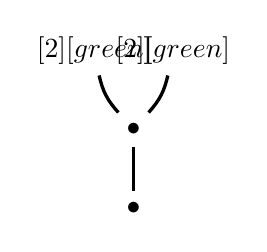
\begin{tikzpicture}[very thick, scale=0.5]
\node (foot) at (2,0) {$\bullet$};
\node (N1) at (2,2) {$\bullet$};
\node (N2) at (3,4) {$\Smiley[2][green]$};
\node (N3) at (1,4) {$\Smiley[2][green]$};
\draw (foot) -- (N1);
\draw (N1) to [bend right =15] (N2);
\draw (N1) to  [bend left=15](N3);
\end{tikzpicture}
\caption{\label{fig:HM}}
The state of the hydra after $M$ rounds.
% The hydra \texttt{h} of the proof that \(\omega^2\) is too small for proving Hercules' victory

\end{figure}


\begin{figure}[htb]
\centering
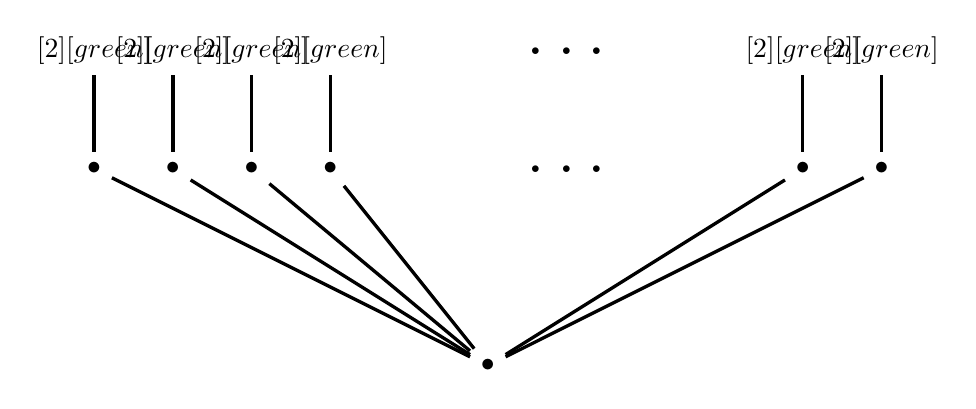
\begin{tikzpicture}[very thick, scale=0.5]
\node (foot) at (10,0) {$\bullet$};
\node (N1) at (0,5) {$\bullet$};
\node (N12) at (0,8) {$\Smiley[2][green]$};
\node (N2) at (2,5) {$\bullet$};
\node (N22) at (2,8) {$\Smiley[2][green]$};
\node (N3) at (4,5) {$\bullet$};
\node (N32) at (4,8) {$\Smiley[2][green]$};
\node (N4) at (6,5) {$\bullet$};
\node (N42) at (6,8) {$\Smiley[2][green]$};

\node (Ndots) at (12,8) {\Huge $\dots$};
\node (Ndots2) at (12,5) {\Huge $\dots$};

\node (N8) at (18,5) {$\bullet$};
\node (N82) at (18,8) {$\Smiley[2][green]$};
\node (N9) at (20,5) {$\bullet$};
\node (N92) at (20,8) {$\Smiley[2][green]$};


\draw (foot) -- (N1);
\draw (foot) -- (N2);
\draw (foot) -- (N3);
\draw (foot) -- (N4);
\draw (foot) -- (N8);
\draw (foot) -- (N9);
\draw (N1) to  (N12);
\draw (N2) to  (N22);
\draw (N3) to  (N32);
\draw (N4) to  (N42);
\draw (N8) to  (N82);
\draw (N9) to  (N92);
\end{tikzpicture}
\caption{\label{fig:HM-plus1}}
The state of the hydra after $M+1$ rounds (with $M+1$ heads). 

\end{figure}


\input{movies/snippets/BigBattle/L295S}

\vspace{4pt}

Then, applying once more the lemma \texttt{BigStep}, we get the exact time when
Hercules wins!

\vspace{4pt}

\input{movies/snippets/BigBattle/NDef}

\vspace{4pt}

We are now able to prove formally that the considered battle is 
composed of $N$ steps.

\vspace{4pt}

\input{movies/snippets/BigBattle/Done}


\subsection{A minoration lemma}

Now, we would like to get an intuition of  how big the number $N$ is.
For that purpose, we use a minoration of the function \texttt{doubleS} by the
function (\texttt{fun n => 2 * n}).

\vspace{4pt}

\input{movies/snippets/Exp2/exp2Def}

\vspace{4pt}

Using a few facts (proven in 
\href{../theories/html/hydras.Hydra.BigBattle.html}{hydras.Hydra.BigBattle}),we get several  minorations.

\input{movies/snippets/BigBattle/minorationLemmas}

\vspace{4pt}


The number $N$ is greater than or  equal to $2^{2^{95}\times 95}.$ If we wrote $N$ in base $10$, $N$ would require at least $10^{30}$ digits!


\section{Generic properties}


The example we just studied shows that the termination of any battle may take a very long time. If we want to study hydra battles in general, we have to consider 
any hydra and any strategy, both for Hercules and the hydra itself. So, we first  give some definitions, generally borrowed from transition systems vocabulary (see~\cite{tel_2000} for instance).


\subsection{Liveliness}


Let $B$ be an instance of \texttt{Battle}. We say that $B$ is \emph{alive} if
for any configuration $(i,h)$, where $h$ is not a head, there exists a further step in class $B$.


\vspace{4pt}
\emph{From Module~\href{../theories/html/hydras.Hydra.Hydra_Definitions.html\#Alive}{Hydra.Hydra\_Definitions}}

\input{movies/snippets/Hydra_Definitions/AliveDef}


The theorems \texttt{Alive\_free} and \texttt{Alive\_standard} of the module 
\href{../theories/html/hydras.Hydra.Hydra_Theorems.html}{Hydra.Hydra\_Theorems} show that the classes \texttt{free} and \texttt{standard} satisfy this property.

\vspace{4pt}
\emph{From Module~\href{../theories/html/hydras.Hydra.Hydra_Lemmas.html\#next_round_dec}{Hydra.Hydra\_Lemmas}}

\input{movies/snippets/Hydra_Lemmas/nextRoundDec}

\emph{From Module~\href{../theories/html/hydras.Hydra.Hydra_Theorems}{Hydra.Hydra\_Theorems}}

\input{movies/snippets/Hydra_Theorems/AliveThms}



\subsection{Termination}

The termination of \emph{any}  battle is naturally expressed by the predicate \texttt{well\_founded} defined in the module \href{https://coq.inria.fr/distrib/current/stdlib/Coq.Init.Wf.html}{Coq.Init.Wf} 
 of the Standard Library.

\index{hydras}{Library Hydra!Predicates!Termination}

\input{movies/snippets/Hydra_Definitions/TerminationDef}



Let $B$ be an instance of class \texttt{Battle}. A \emph{variant} for $B$ consists
in a well-founded relation $<$  on some type \texttt{A}, and a function
(also called a \emph{measure}) $m:\texttt{Hydra}\rightarrow A$ such that for any successive steps $(i,h)$ and $(1+i,h')$  of a battle in $B$, the inequality $m(h')<m(h)$ holds.


\vspace{4pt}
\noindent

\emph{From Module~\href{../theories/html/hydras.Hydra.Hydra_Definitions.html\#Hvariant}{Hydra.Hydra\_Definitions}}


\label{sect:hvariant-def}

\index{hydras}{Library Hydra!Type classes!Hvariant}

\input{movies/snippets/Hydra_Definitions/HvariantDef}

\index{hydras}{Exercises}

\begin{exercise}
 Prove that, if there exists some  instance of (\texttt{Hvariant Lt wf\_Lt $B$ $m$}), then there exists no infinite battle in  $B$.
\end{exercise}




\subsection{A  small proof of impossibility}
%\index{coq}{Proofs of impossibility}

\label{omega-case}

When one wants to prove a termination theorem with the help of a variant, 
one has to consider first a well-founded set $(A,<)$, then a strictly decreasing measure on this set.  The following  lemma shows that,  if  the order structure $(A,<)$ is too simple, it is useless to look for a convenient measure, which simply no exists. Such kind of result is useful, because it saves you time and effort.


The best known well-founded order is the natural order on the set $\mathbb{N}$ of natural numbers (the type \texttt{nat} of Standard library). It would be interesting to look for some measure $m:\texttt{nat}\arrow\texttt{nat}$ and prove it is a variant.

Unfortunately, we can prove that 
\emph{no} instance of class (\texttt{WfVariant round Peano.lt $m$}) can be built, where
$m$ is \emph{any} function of type \texttt{Hydra $\arrow$ nat}.


Let us present the main steps of that proof, the script of which  is in the module ~\href{../theories/html/hydras.Hydra.Omega_Small.html}{Hydra/Omega\_Small.v} \footnote{ The name of this file means ``the ordinal $\omega$ is too small for proving the termination of [free] hydra battles ''. In effect, the elements of $\omega$, considered as a set, are just the natural numbers (see next chapter for more details)}.

%\subsubsection{Preliminaries}


Let us assume there exists some variant $m$ from \texttt{Hydra} into (\texttt{nat},$<$)  for proving
    the  termination of all hydra battles.

\input{movies/snippets/Omega_Small/omegaSmalla}
    
We define an injection $\iota$ from the type \texttt{nat} into \texttt{Hydra}.
For any natural number $i$, $\iota(i)$ is the hydra composed of a foot and
$i+1$ heads at height $1$. For instance, Fig.~\ref{fig:flower} represents the hydra $\iota(3)$.

\begin{figure}[htb]
\centering
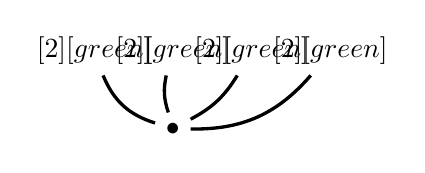
\begin{tikzpicture}[very thick, scale=0.5]
\node (foot) at (4,0) {$\bullet$};
\node (N1) at (2,2) {$\Smiley[2][green]$};
\node (N2) at (4,2) {$\Smiley[2][green]$};
\node (N3) at (6,2) {$\Smiley[2][green]$};
\node (N4) at (8,2) {$\Smiley[2][green]$};
\draw (foot) to [bend left =25] (N1);
\draw (foot) to [bend left =15] (N2);
\draw (foot) to [bend right =15] (N3);
\draw (foot) to [bend right =25] (N4);
\end{tikzpicture}
\caption{\label{fig:flower}
The hydra $\iota(3)$}
\end{figure}

\input{movies/snippets/Omega_Small/iotaDef}

Let us consider now some hydra \texttt{big\_h} out of the range of the injection $\iota$ (see Fig.~\vref{fig:h-omega-omega}).

\begin{figure}[htb]
\centering
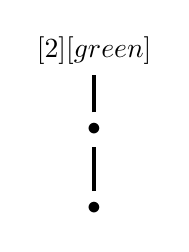
\begin{tikzpicture}[very thick, scale=0.5]
\node (foot) at (2,0) {$\bullet$};
\node (N1) at (2,2) {$\bullet$};
\node (N2) at (2,4) {$\Smiley[2][green]$};
\draw (foot) -- (N1);
\draw (N1) to  (N2);
\end{tikzpicture}
\caption{\label{fig:h-omega-omega}}
 The hydra \texttt{big\_h}.
\end{figure}

\input{movies/snippets/Omega_Small/bigHDef}


 Using the functions $m$ and $\iota$, we define a second hydra \texttt{small\_h}, and show
 there is a one-round battle that transforms \texttt{big\_h} into \texttt{small\_h}. Please note that,
due to the hypothesis \texttt{Hvar}, we are interested in the termination of \emph{free} battles. 
There is no problem to consider a round with (\texttt{m big\_h}) as the replication factor.


\input{movies/snippets/Omega_Small/smallHDef}


 
But, by hypothesis, $m$ is a variant. Hence, we infer the following inequality.

\vspace{4pt}

\input{movies/snippets/Omega_Small/mLt}


In order to get a contradiction, it suffices to  prove the inequality
$m(\texttt{big\_h}) \leq m(\texttt{small\_h})$ i.e.,  $m(\texttt{big\_h}\leq m(\iota (m(\texttt{big\_h})))$.


\input{movies/snippets/Omega_Small/mGea}


Intuitively, it means that, from any hydra of the form (\texttt{iota $i$}), the battle will 
take (at least) $i$ rounds. Thus the associated measure cannot be less than $i$.
Technically, we prove this lemma by Peano induction on $i$.

\begin{itemize}
\item The base case $i=0$ is trivial
\item Otherwise, let $i$ be any natural number and assume  the inequality
  $i \leq m(\iota(i))$.
  \begin{enumerate}
  \item  But the hydra $\iota(S(i))$ can be transformed in one round into
    $\iota(i)$ (by losing its rightmost head, for instance)
  \item Since $m$ is a variant, we have $m(\iota(i)) < m(\iota(S(i)))$,
    hence  $i< m(\iota(S(i)))$, which implies  $S(i)\leq  m(\iota(S(i)))$.
  \end{enumerate}
\end{itemize}

We are now ready to complete our impossibility proof.

\vspace{4pt}

\inputsnippets{Omega_Small/mGeb, Omega_Small/mGez,
  Omega_Small/omegaSmallz}
 


\index{hydras}{Exercises}

\begin{exercise}
Prove that there exists no variant $m$ from \texttt{Hydra} into \texttt{nat} for proving
    the  termination of all \emph{standard} battles.
\end{exercise}






\subsubsection{Conclusion}

In order to build a variant for proving the termination of all hydra battles, we need to consider order structures more complex than the usual order on type \texttt{nat}. 
The notion of \emph{ordinal number} provides a catalogue of well-founded order types.
For a reasonably large bunch of ordinal numbers, \emph{ordinal notations} are data-types which allow the \coq{} user to define functions, to compute and prove some properties, for instance by reflection.

The next chapter is dedicated to a generic formalization of ordinal notations, and chapter~\ref{chap:T1} to a proof of termination of all hydra battles with the help of an ordinal notation for the interval $[0,\epsilon_0)$\,\footnote{We use the mathematical notation $[a,b)$ for the interval $\{x|a\leq x < b\}$.}.
\index{maths}{Notations!Interval}
